%% if you are submitting an initial manuscript then you should have submission as an option here
%% if you are submitting a revised manuscript then you should have revision as an option here
%% otherwise options taken by the article class will be accepted
\documentclass[submission]{FPSAC2021}
%% but DO NOT pass any options (or change anything else anywhere) which alters page size / layout / font size etc

%% note that the class file already loads {amsmath, amsthm, amssymb}


\usepackage{mathtools}
\usepackage[all]{xy}
\usepackage[vcentermath]{youngtab}



\theoremstyle{plain}
\newtheorem{theorem}{Theorem}[section]
\newtheorem{proposition}[theorem]{Proposition}
\newtheorem{claim}[theorem]{Claim}
\newtheorem{lemma}[theorem]{Lemma}
\newtheorem{corollary}[theorem]{Corollary}
\newtheorem{conjecture}[theorem]{Conjecture}
\newtheorem{problem}[theorem]{Problem}

%\theoremstyle{definition}
\newtheorem{definition}[theorem]{Definition}
\newtheorem{examplex}[theorem]{Example}
\newenvironment{example}
 {\pushQED{\qed}\examplex}
  {\popQED\endexamplex}
\newtheorem{remark}[theorem]{Remark}
\newtheorem{case}{Case}



\numberwithin{equation}{section}

%%%% commenting %%%%
\newcommand{\JL}[1]{{\color{blue} JL: #1}}
\newcommand{\SG}[1]{{\color{red} SG: #1}}
\newcommand{\AW}[1]{{\color{green} AW: #1}}


%%%% blackboard letters %%%%

\newcommand{\bC}{\mathbb{C}}
\newcommand{\bN}{\mathbb{N}}
\newcommand{\bK}{\mathbb{K}}
\newcommand{\bP}{\mathbb{P}} 
\newcommand{\bQ}{\mathbb{Q}}
\newcommand{\bR}{\mathbb{R}}
\newcommand{\bZ}{\mathbb{Z}}

%%%%% calligraphic commands %%%%

\newcommand{\cA}{\mathcal{A}}
\newcommand{\cB}{\mathcal{B}}
\newcommand{\cC}{\mathcal{C}}
\newcommand{\cF}{\mathcal{F}}
\newcommand{\cG}{\mathcal{G}}
\newcommand{\cI}{\mathcal{I}}
\newcommand{\cJ}{\mathcal{J}}
\newcommand{\cK}{\mathcal{K}}
\newcommand{\cL}{\mathcal{L}}
\newcommand{\cN}{\mathcal{N}}
\newcommand{\cP}{\mathcal{P}}
\newcommand{\cW}{\mathcal{W}}

%%%%% fraktur commands %%%%%

\newcommand{\fg}{\mathfrak{g}}
\newcommand{\fh}{\mathfrak{h}}
\newcommand{\fS}{\mathfrak{S}}
\newcommand{\fC}{\mathfrak{C}}


%%%%% some color macros  %%%%%

\newcommand{\tcr}[1]{\textcolor{red}{#1}}
\newcommand{\tcb}[1]{\textcolor{blue}{#1}}
\newcommand{\tcg}[1]{\textcolor{green}{#1}}
\newcommand{\tcc}[1]{\textcolor{cyan}{#1}}
\newcommand{\tcm}[1]{\textcolor{magenta}{#1}}
\newcommand{\tcp}[1]{\textcolor{purple}{#1}}

%%%%% derivative macros %%%%%

\newcommand{\der}[2][]{\frac{d#1}{d#2}}
\newcommand{\pder}[2][]{\frac{\partial#1}{\partial#2}}

%%%% combinatorics statistics %%%%%

\newcommand{\des}{\mathrm{des}}
\newcommand{\asc}{\mathrm{asc}}
\newcommand{\Des}{\mathrm{Des}}
\newcommand{\Asc}{\mathrm{Asc}}



%%%% algebra macros %%%%

\newcommand{\gr}{\mathrm{gr}}
\newcommand{\hgr}{\mathrm{hgr}} %homogeneous grading, used in tree symm paper follow-up
\newcommand{\vecspan}{\mathrm{span}}
\newcommand{\ch}{\mathrm{ch}}
\newcommand{\grch}{\mathrm{grch}} %graded Frob. characteristic, used in tree symm paper follow-up

\renewcommand{\top}{\mathrm{top}}
\newcommand{\std}{\mathrm{std}}
\newcommand{\conv}{\mathrm{conv}}
\newcommand{\sch}{\mathfrak{S}}
\newcommand{\init}{\mathrm{init}}
\newcommand{\Inv}{\mathrm{Inv}}
\newcommand{\st}{\,:\,}
\newcommand{\vspan}{\mathrm{span}}
\newcommand{\bA}{\mathbb{A}}
\newcommand{\Fl}{\mathrm{Fl}}
\newcommand{\Hilb}{\mathrm{Hilb}}
\newcommand{\Frob}{\mathrm{Frob}}
\newcommand{\la}{\lambda}
\newcommand{\im}{\mathrm{im}}
\newcommand{\SYT}{\mathrm{SYT}}
\newcommand{\sort}{\mathrm{sort}}
\newcommand{\fl}{\mathrm{fl}}
\newcommand{\ufl}{\mathrm{ufl}}
\newcommand{\inv}{\mathrm{inv}}




\usepackage{lipsum}


%% define your title in the usual way
\title{Springer fibers and the Delta Conjecture at $t=0$}

%% define your authors in the usual way
%% use \addressmark{1}, \addressmark{2} etc for the institutions, and use \thanks{} for contact details
%%\author[Optional shorter names]{Longer names me\thanks{\href{mailto:hello@world.c}{hello@world.c}. Longer names me was partially supported by Grant 2017.11.14.$\partial$\;supp.}\addressmark{1}, \and you\addressmark{2}}

%\author{Sean T. Griffin\thanks{\href{mailto:segriffin@ucsd.edu}{segriffin@ucsd.edu}}
%\addressmark{1}, Jake Levinson\addressmark{2}, \and Alexander Woo\addressmark{3}}

\author{Sean T. Griffin\thanks{\href{mailto:segriffin@ucsd.edu}{segriffin@ucsd.edu}}\addressmark{1}, \and Jake Levinson\thanks{\href{mailto:jake_levinson@sfu.ca}{jake\_levinson@sfu.ca} Jake Levinson was partially supported by an AMS Simons Travel Grant}, \and Alexander Woo\thanks{\href{mailto:awoo@uidaho.edu}{awoo@uidaho.edu}.  Alexander Woo was partially supported by Simons Collaboration Grant 359792}}

%% then use \addressmark to match authors to institutions here
\address{\addressmark{1}Department of Mathematics, University of California, San Diego, La Jolla, CA, USA \\ \addressmark{2}Department of Mathematics, Simon Fraser University, Burnaby, BC, Canada \\\addressmark{3}Department of Mathematics and Statistical Science, University of Idaho, Moscow, ID, USA}

%% put the date of submission here
\received{December 1, 2020}

%% leave this blank until submitting a revised version
%\revised{}

%% put your English abstract here, or comment this out if you don't have one yet
%% please don't use custom commands in your abstract / resume, as these will be displayed online
%% likewise for citations -- please don't use \cite, and instead write out your citation as something like (author year)
\abstract{We define a family of varieties $Y_{n,\lambda,s}$ generalizing the type A Springer fibers, whose cohomology rings have the structure of an $S_n$-module. We give an explicit presentation for the cohomology ring $H^*(Y_{n,\lambda,s};\bQ)$, and we find an affine paving of $Y_{n,\lambda,s}$ that is in bijection with a collection of partial row-strict fillings of a partition shape. We also prove that the top cohomology groups of $Y_{n,\lambda,s}$ give a generalization of the type A Springer correspondence to the setting of induced Specht modules.
Furthermore, the special case $Y_{n,(1^k),k}$ of our variety gives a new geometric realization of the representation corresponding to the expression in the Delta Conjecture when $t=0$. 
}

%% put your French abstract here, or comment this out if you don't have one
\resume{Nous introduisons une famille de vari\'et\'es $Y_{n,\lambda,s}$ qui g\'en\'eralise les fibres de Springer pour $SL_n$, dont les anneaux de cohomologie sont des repr\'esentations de $S_n$. Nous fournissons une pr\'esentation explicite pour ces anneaux de cohomologie, ainsi qu'une pavage d'affines en bijection avec une collection de tableaux strictement d\'ecroissantes dans les lignes.  Nous d\'emontrons aussi que les groupes de cohomologie de degr\'e maximum de $Y_{n,\lambda,s}$ sont les repr\'esentations induites des repr\'esentations irr\'eductibles de $S_n$; ceci g\'en\'eralise la correspondance de Springer.  De plus, pour $\lambda=1^k$, la vari\'et\'e $Y_{n,(1^k),k}$ fournit une r\'ealisation g\'eom\'etrique nouvelle de la repr\'esentation correspondant \'a l'expression de la conjecture delta pour $t=0$.}

%% put your keywords here, or comment this out if you don't have them yet
\keywords{Springer fiber, cohomology, affine paving, Specht module, symmetric function, ordered set partition}

%% you can include your bibliography however you want, but using an external .bib file is STRONGLY RECOMMENDED and will make the editor's life much easier
%% regardless of how you do it, please use numerical citations, ie. [xx, yy] in the text

%% this sample uses biblatex, which (among other things) takes care of URLs in a more flexible way than bibtex
%% but you can use bibtex if you want
\usepackage[backend=bibtex]{biblatex}
\addbibresource{Springer.bib}
%% note the \printbibliography command at the end of the file which goes with these biblatex commands

\begin{document}

\maketitle
%% note that you DO NOT have to put your abstract here -- it is generated by \maketitle and the \abstract and \resume commands above

\section{Introduction}

In this article, we introduce a family of varieties generalizing the Springer fibers. We find an explicit presentation of their cohomology rings generalizing the one given by Tanisaki for the cohomology ring of a Springer fiber~\cite{Tanisaki}. This presentation coincides with the graded ring introduced and studied by the first author~\cite{GriffinOSP}.  As a special case, our construction gives a new \emph{compact} geometric realization of the  expression in the Delta Conjecture in the case $t=0$. We also prove a version of the Springer correspondence for this family of varieties, showing that their top cohomology groups have the $S_n$-module structure of an induced Specht module.



In the seminal work~\cite{Springer-WeylGrpReps,Springer-TrigSum}, T.A. Springer introduced a family of varieties associated to any complete flag variety $G/B$, called Springer fibers, that have remarkable connections to the representation theory of the corresponding Weyl group. Springer proved that although the Weyl group does not act on a Springer fiber, it does act nontrivially on the cohomology ring of a Springer fiber. In type A, the Weyl group is the symmetric group $S_n$. Springer proved that the highest degree nonzero cohomology group of a Springer fiber is an irreducible representation of $S_n$, and every irreducible representation appears this way. This is known as the \emph{Springer correspondence}. We note that the $S_n$-action discussed in this paper differs from Springer's original construction by tensoring with the sign representation.

The graded $S_n$-module type of the cohomology ring of a Springer fiber was discovered by Hotta and Springer~\cite{Hotta-Springer}. Under the Frobenius characteristic map $\Frob$ that associates a symmetric function to each $S_n$-module, the cohomology ring of a Springer fiber is sent to the \emph{modified Hall-Littlewood symmetric function}
\begin{align}
\Frob(H^*(\cB^\lambda;\bQ);q) = \widetilde H_\lambda(x;q^2),
\end{align}
where the $q$ on the left-hand side keeps track of the grading of the cohomology ring. The cohomology ring of a Springer fiber was made explicit by De Concini--Procesi~\cite{dCP} and Tanisaki~\cite{Tanisaki}, who found quotient ring presentations for $H^*(\cB^\lambda;\bQ)$. These presentations generalize Borel's theorem that the cohomology of $\Fl(n)$ is the type A coinvariant ring.
A detailed analysis of the graded Frobenius characteristic of the cohomology ring was then given by Garsia and Procesi~\cite{Garsia-Procesi}, who were inspired by these presentations.

The Delta Conjecture of Haglund--Remmel--Wilson~\cite{HRW}, recently proved by D'Adderio and Mellit~\cite{DM}, gives a combinatorial formula for a symmetric function, $\Delta'_{e_{k-1}} e_n(q, t)$, coming from the theory of Macdonald polynomials. Since $\Delta'_{e_{k-1}} e_n(q,t)$ is conjectured to be Schur-positive, there is much interest in a natural algebraic or geometric construction of a (bigraded) $S_n$-module whose Frobenius characteristic is $\Delta'_{e_{k-1}} e_n(q,t)$. Haglund--Rhoades--Shimozono~\cite{HRS1} did this in the case $t=0$ by constructing a graded ring $R_{n,k}$ with a suitable $S_n$-action whose graded Frobenius characteristic is $\Delta'_{e_{k-1}} e_n(q, 0)$ (after a minor twist). The ring $R_{n,k}$ is defined as
\begin{align}
    R_{n,k}\coloneqq \frac{\bQ[x_1,\dots,x_n]}{\langle x_1^k,\dots, x_n^k,e_n,e_{n-1},\dots, e_{n-k+1}\rangle}
\end{align}
and specializes to the type A coinvariant ring in the case $n=k$. 

Pawlowski and Rhoades~\cite{Pawlowski-Rhoades} gave a parallel geometric interpretation by exhibiting a variety whose cohomology ring is $R_{n,k}$.  They defined the space of \emph{spanning line arrangements}, $n$-tuples of lines in $\bC^k$ that span $\bC^k$,
\begin{align}
X_{n,k} \coloneqq \{(L_1,\dots, L_n) \in (\bP^{k-1})^n \st L_1+\cdots +L_n = \bC^k\}.
\end{align}
Unlike Springer fibers, which are closed subvarieties of $\Fl(n)$, the space $X_{n,k}$ is an open subvariety of the product space $(\bP^{k-1})^n$, and hence $X_{n,k}$ is smooth and noncompact in general.
Pawlowski and Rhoades proved that 
\begin{align}
H^*(X_{n,k};\bQ) \cong R_{n,k},
\end{align}
thus giving a connection between the expression in the Delta Conjecture at $t=0$ and geometry. 

Since the Poincare series recording the graded dimensions of the ring $R_{n,k}$ is not symmetric, then by Poincare duality, any complex variety whose cohomology ring is isomorphic to $R_{n,k}$ must either be noncompact or singular. In this article, we introduce a compact and singular variety $Y_{n,(1^k),k}$, similar to a Springer fiber, whose cohomology ring is the Haglund--Rhoades--Shimozono ring $R_{n,k}$. 
The space $Y_{n,(1^k),k}$ is constructed as a closed subvariety of a partial flag variety, and it naturally embeds into an iterated projective bundle whose cohomology ring is isomorphic to the cohomology ring of the product space $(\bP^{k-1})^n$.
 Furthermore, the variety $Y_{n,(1^k),k}$ fits into a larger family of varieties $Y_{n,\lambda,s}$, indexed by integers $n$ and $s$ and partitions $\lambda$ of size $k\leq n$, that contains the Springer fiber $\cB^\lambda$ as a special case. 


%\JL{Might be nice to spell out / mention that a product of projective spaces clearly has the correct cohomology for the base case, making it a natural starting guess for a family of compact varieties. But, instead we use this twisted bundle with the same cohomology.}




As our main result, we prove an explicit presentation of the ring $H^*(Y_{n,\la,s};\bQ)$ as a quotient of a polynomial ring, generalization Tanisaki's presentation for the cohomology ring of a Springer fiber~\cite{Tanisaki}. This presentation coincides with the graded ring $R_{n,\lambda,s}$ recently introduced by the first author~\cite{GriffinOSP}. 
As a consequence, we see that the cohomology ring of $Y_{n,\lambda,s}$ has a graded $S_n$-module structure generalizing the classical one in the Springer fiber case.

One of our main tools for proving our presentation of the cohomology ring is an affine paving  of $Y_{n,\lambda,s}$, which allows us to compute the ranks of the cohomology groups. The cells in our affine paving are in bijection with ordered set partitions $(B_1|\cdots|B_s)$ of $[n]$ such that $|B_i|\geq \lambda_i$. Equivalently, the cells are in bijection with certain row strict fillings whose shape contains $\lambda$. The irreducible components of the variety $Y_{n,\lambda,s}$ are the cell closures corresponding to row strict fillings in which the restriction of the labeling to $\lambda$ standardizes to a standard Young tableau and such that all of the labels not in $\lambda$ are in the lowest row.

We use results of the first author to prove a generalization of the  Springer correspondence to the setting of induced Specht modules. We show that for general $s$, the top cohomology group of $Y_{n,\lambda,s}$ is isomorphic as an $S_n$-module to the irreducible $S_k$-module $S^\lambda$ induced up to $S_n$.
%We show that for $s>\ell(\lambda)$, 
%\begin{align}
%H^{2d}(Y_{n,\lambda,s};\bQ) \cong \mathrm{Ind}\!\uparrow_{S_k}^{S_n} (S^\lambda),
%\end{align}
%where $d$ is the dimension of the variety $Y_{n,\lambda,s}$ and $S^\la$ is the irreducible Specht module indexed by $\lambda$. In the special case when $s=\ell(\lambda)$, we show that the top cohomology group is a skew Specht module $S^{\Lambda/(n-k)^{s-1}}$. 
%We also prove that $Y_{n,\lambda,s}$ is equidimensional,
%of dimension
%\begin{align}
%    d = \sum_i \binom{\lambda_i'}{2} + (s-1)(n-k),
%\end{align}
%and we give a characterization of the irreducible components of $Y_{n,\la,s}$.
%\SG{Spell out the combinatorics of the affine paving and which cells correspond to irreducible components.}

In Section~\ref{sec:SpringerFibers}, we recall the Springer fibers and their connections to representation theory.
In Section~\ref{sec:YVarieties}, we define the variety $Y_{n,\lambda,s}$ and state our main theorem, which is an explicit presentation of the cohomology ring of $Y_{n,\lambda,s}$ which allows us to define an $S_n$-action on the cohomology ring.
In Section~\ref{sec:AffinePaving}, we construct an affine paving of $Y_{n,\lambda,s}$, which is one of our main tools in proving the presentation of the cohomology ring.
In Section~\ref{sec:InducedSpecht}, we prove our generalization of the Springer correspondence, and we characterize the irreducible components of the variety $Y_{n,\la,s}$.
Finally, in Section~\ref{sec:FutureWork} we list some open problems.


\section{Springer fibers}\label{sec:SpringerFibers}

Given a partition $\lambda$ of $n$, let $N$ be a $n\times n$ nilpotent matrix whose Jordan block sizes are recorded by $\lambda$. The {\bf Springer fiber} associated to $\lambda$ is
\begin{align}
    \cB^\lambda \coloneqq \{V_\bullet \in \Fl(n) \st NV_i\subseteq V_i \text{ for all } i\leq n\}.
\end{align}
Springer proved that although $S_n$ does not act on $\cB^\lambda$, it does act on the cohomology ring of $\cB^\lambda$. We note that in this article, the action on the cohomology ring we consider differs from the one originally constructed by Springer by tensoring with the sign representation.

A remarkable property of this action is that the top nonzero cohomology groups of $\cB^\lambda$ give a geometric construction of the irreducible Specht modules.
\begin{theorem}[Springer]
In Lie type A there is a bijection, known as the Springer correspondence, between Springer fibers and the irreducible $S_n$-modules, up to isomorphism.  Specifically, the top nonzero cohomology group of $\cB^\lambda$ as an $S_n$-module is
\begin{align}
    H^{2n(\lambda)}(\cB^\lambda;\bQ) \cong S^\lambda,
\end{align}
where 
\begin{align}
    n(\lambda) \coloneqq \sum_i \binom{\lambda_i'}{2} = \dim_\bC(\cB^\lambda).
\end{align}
\end{theorem}

Hotta and Springer~\cite{Hotta-Springer} proved that the map on cohomology induced by the inclusion $\cB^\lambda \subseteq \Fl(n)$,
\begin{align}
    H^*(\Fl(n)) \to H^*(\cB^\lambda),
\end{align}
is surjective. Hence, the cohomology ring $H^*(\cB^\lambda)$ is generated by the cohomology classes $x_i = - c_1(\widetilde V_i/\widetilde V_{i-1})$. Here, we are abusing notation and writing $\widetilde V_i$ for the restriction of this vector bundle to $\cB^\lambda$. 

There is an explicit presentation of $H^*(\cB^\lambda)$ as a quotient ring extending Borel's theorem that the cohomology ring of $\Fl(n)$ is isomorphic to the type A coinvariant ring~\cite{dCP,Tanisaki}. For all $i\leq n$, let $p_i(\lambda) = \la'_n + \la'_{n-1} +\cdots + \la'_{n-i+1}$, where $\la'_i = 0$ for all $i>\la_1$. Given $S\subseteq \{x_1,\dots, x_n\}$, let $e_d(S)$ be the sum of all square-free products of variables in $S$ of degree $d$. The ideal $I_\lambda$ and quotient ring $R_\lambda$ are defined as follows,
\begin{align}
    I_\lambda &\coloneqq \langle e_d(S) \,:\, |S|\geq d > |S| - p_{|S|}(\lambda)\rangle,\\
    R_\lambda &\coloneqq \bQ[x_1,\dots, x_n]/I_\lambda.
\end{align}
Tanisaki~\cite{Tanisaki} proved that there is an isomorphism of graded rings
\begin{align}
    H^*(\cB^\lambda;\bQ) \cong R_\lambda
\end{align}
given by identifying the cohomology class $x_i$ with the variable $x_i$. For example, when $\lambda = (2,1)$, then $p_{1}(\lambda) = 0$, $p_2(\lambda) = 1$, and $p_3(\lambda) = 3$. Therefore, $I_\lambda$ is generated by $e_d(S)$ where $3\geq d>0$ and $|S|=3$, or $2\geq d>1$ and $|S| = 2$, so 
\begin{align}
I_{(2,1)} = \langle e_1(x_1,x_2,x_3), e_2(x_1,x_2,x_3), e_3(x_1,x_2,x_3), e_2(x_1,x_2), e_2(x_1,x_3), e_2(x_2,x_3)\rangle.
\end{align}
and $H^*(\cB^{(2,1)};\bQ)\cong \bQ[x_1,x_2,x_3]/I_{(2,1)}$.







\section{The variety $Y_{n,\lambda,s}$}\label{sec:YVarieties}

The variety $Y_{n,\lambda,s}$ is defined as follows. Fix integers $0\leq k\leq n$ (with $n>0$), a partition $\lambda\vdash k$, and an integer $s\geq \ell(\lambda)$. Define $m = k + s(n-k)$, and let $\Fl_{1,\dots, n}(\bC^m)$ be the partial flag variety of ascending chains of subspaces $V_1\subset V_2\subset \cdots \subset V_n\subset \bC^m$ with $\dim_\bC(V_i) = i$ for all $i$. 

Fix a nilpotent endomorphism $N$ of $\bC^m$ whose matrix has Jordan type $\Lambda = (n-k+\la_1,n-k+\la_2,\dots, n-k+\la_s)$, where $\la_i \coloneqq 0$ for $i>\ell(\la)$, see Figure~\ref{fig:Lambda}. Define $\bC^\lambda \coloneqq \im(N^{n-k})$, which a subspace on which $N$ has Jordan type $\lambda$. We define the following variety, which is our main object of study
\begin{align}
Y_{n,\la,s} \coloneqq \{V_\bullet \in \Fl_{1,\dots, n}(\bC^m) \st N V_i\subseteq V_{i-1}\text{ for all }i,\text{ and } V_n\supseteq \bC^\lambda\}.
\end{align}
\begin{figure}
    \centering
    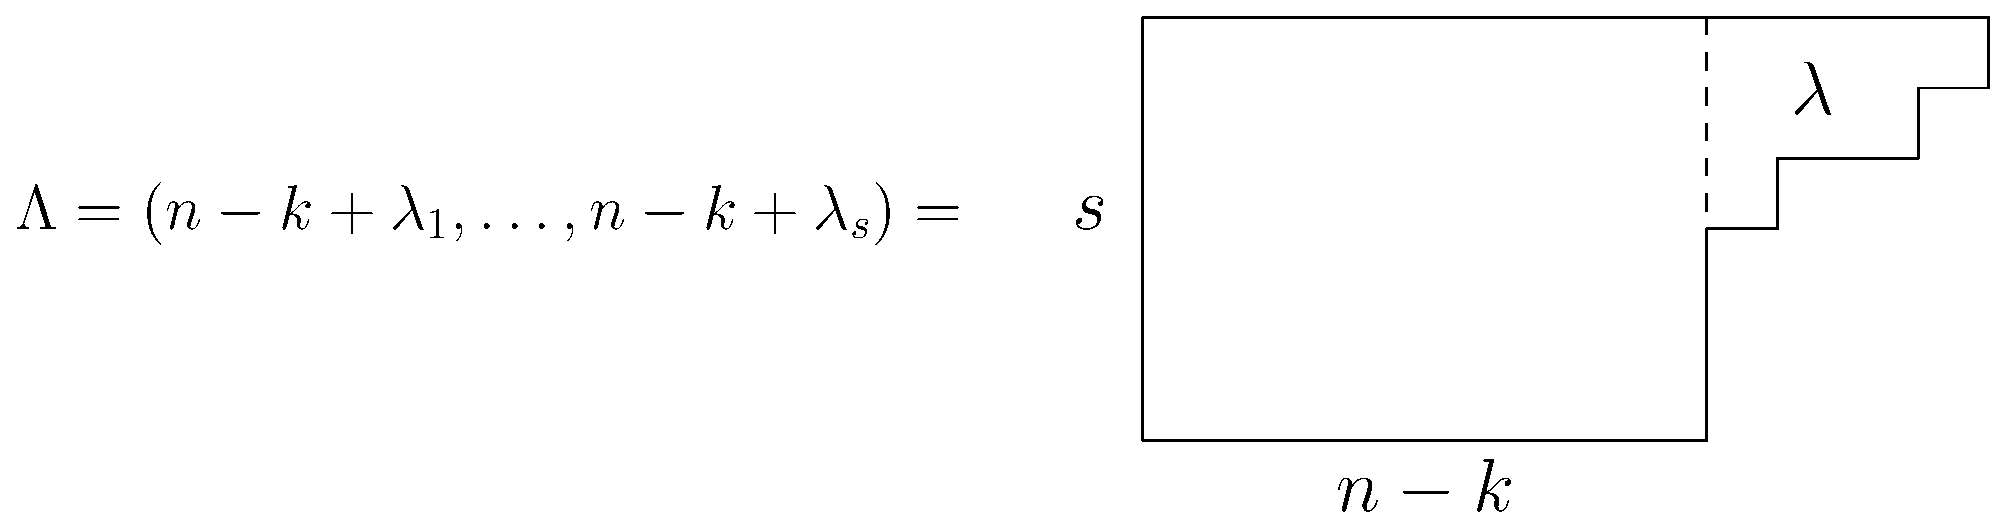
\includegraphics[width=0.8\textwidth]{LambdaEx.eps}
    \caption{The partition $\Lambda$ representing the Jordan type of $N$.
    %The maximal cells correspond to flags inducing a particular Jordan type on the nilpotent operator $N$.
    }
    \label{fig:Lambda}
\end{figure}


Throughout the paper, we fix a basis of $\bC^m$,
\begin{align}
\{f_{i,j} \st i\leq s,\, j\leq \la_i+n-k\},
\end{align}
 such that $Nf_{i,j} = f_{i,j-1}$ for all $j>1$ and $Nf_{i,1} = 0$. The set of vectors $\{f_{i,j}\}$ is called a \textbf{generalized eigenbasis of $N$}, and the span of the vectors $f_{i,j}$ for a fixed $i$ is called a \textbf{generalized eigenspace of $N$}. Note that $\bC^\lambda = \vspan\{ f_{i,j} \st j \leq \la_i \}$.
 
 \begin{example}
When $k=n$, then it can be checked that $Y_{n,\lambda,s} = \cB^\lambda$ for any $s\geq \ell(\la)$, so these varieties generalize the Springer fibers.\qedhere
 \end{example}
 
\begin{example}
Let $n=5$, $\lambda = (2,1)$, and $s=3$. Then the generalized eigenbasis for the nilpotent operator $N$ can be visualized with the following diagram, where we label the cells in the $i$th row of $\Lambda$ by the vectors $f_{i,n-k+\lambda_i},\dots, f_{i,1}$.
\[
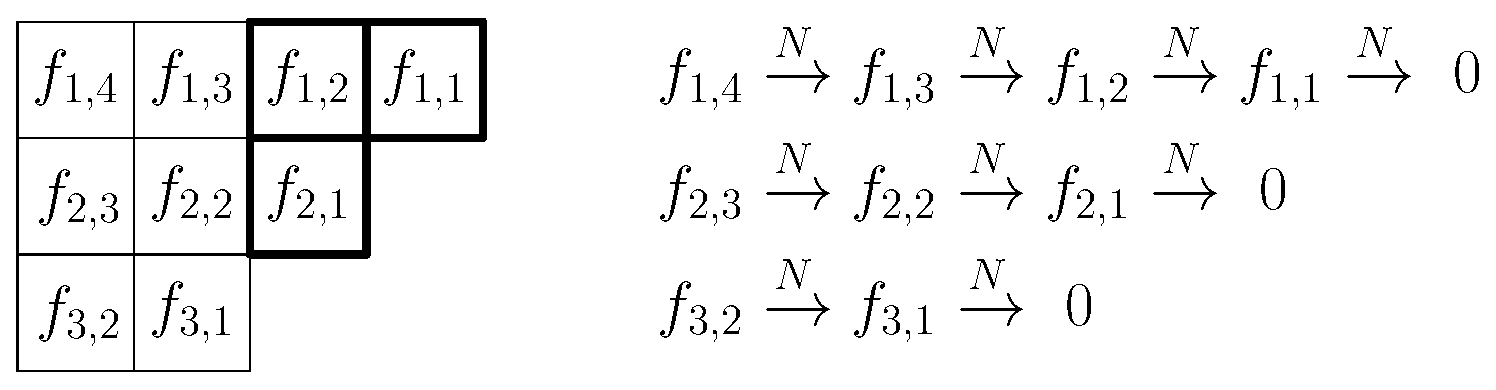
\includegraphics[scale=0.4]{GenEigenbasis.eps}
\]
%\[
%\raisebox{-.8\height}{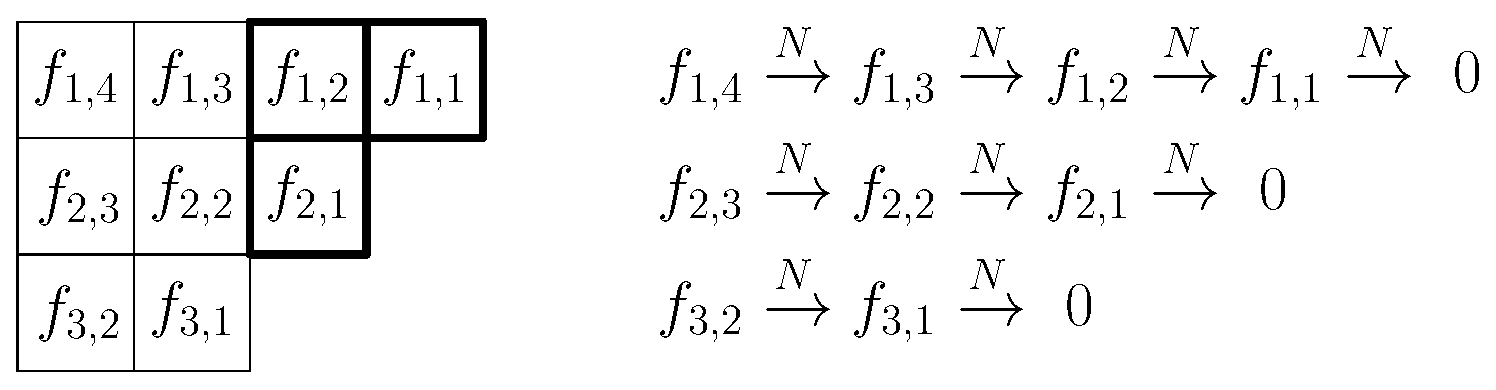
\includegraphics[scale=0.5]{GenEigenbasis.eps}} %\qquad
%\xymatrix{
%f_{1,4} \ar[r]^N & f_{1,3} \ar[r]^N & f_{1, 2} \ar[r]^N & f_{1,1} %\ar[r]^N & 0 \\
%f_{2,3} \ar[r]^N & f_{2,2} \ar[r]^N & f_{2, 1} \ar[r]^N & 0
%\\
%f_{3,2}\ar[r]^N& f_{3,1} \ar[r]^N & 0}
%\]
Notably, $\bC^\lambda = \vspan\{f_{1,1},f_{1,2},f_{2,1}\}$, the span of the vectors contained in the bolded cells with partition shape $(2,1)$. Then $Y_{5,(2,1),3}$ is the variety of partial flags $V_\bullet = (V_1,V_2,V_3,V_4,V_5)\in \Fl_{1,2,3,4,5}(\bC^9)$ such that the following conditions hold:
\begin{align}
N V_i &\subseteq V_{i-1} \text{ for } i \leq 5, \\
% N V_4\subseteq V_3,\, NV_3\subseteq V_2,\, NV_2\subseteq V_1,\, NV_1\subseteq 0,\\
V_5 &\supseteq \vspan\{f_{1,1},f_{1,2},f_{2,1}\}.
\end{align}
For example, the partial flag 
\begin{equation*}\label{eq:PartialFlag}
\langle f_{1, 1} \rangle \subset \langle f_{1,1},f_{1,2} \rangle \subset 
\langle f_{1,1},f_{1,2},f_{3,1} \rangle \subset \langle f_{1,1},f_{1,2},f_{3,1},f_{2,1} \rangle \subset \langle f_{1,1},f_{1,2},f_{3,1},f_{2,1},f_{1,3}\rangle.
\end{equation*}
is in $Y_{5,(2,1),3}$.
\end{example}

Our main result is an explicit presentation of the cohomology ring $H^*(Y_{n,\lambda,s};\bQ)$, which coincides with the quotient ring $R_{n,\lambda,s}$ introduced and studied by the first author in~\cite{GriffinOSP}, which we describe next. Given $n,\la$, and $s$ as above, define 
\begin{align}
    I_{n,\lambda,s} &\coloneqq \langle e_d(S) \,:\, |S|\geq d > |S| - p_{|S|}(\lambda)\rangle + \langle x_i^s \st 1\leq i\leq n\rangle,\\
    R_{n,\lambda,s} &\coloneqq \bQ[x_1,\dots, x_n]/I_{n,\lambda,s}.
\end{align}

\begin{example}
For example, when $n=4$, $\lambda = (2,1)$, and $s=2$, then $I_{4,(2,1),2}$ is generated by $x_i^2$ for $i=1,2,3,4$ and the polynomials 
$e_d(S)$ for $S\subseteq \{x_1,\dots, x_4\}$ such that
\begin{equation*}
\begin{aligned}
	d &= 2 \text{ and }|S| = 4,\\
	d &= 4\text{ and }|S| = 4,\\
\end{aligned}
\qquad
\begin{aligned}
	d &= 3\text{ and }|S| = 4,\\
	d &= 3\text{ and }|S| = 3.
\end{aligned}
\end{equation*}
We have
\begin{align*}
    I_{4,(2,1),2} &= \langle x_1^2,x_2^2,x_3^2,x_4^2,e_2,e_3,e_4,e_3(x_1,x_2,x_3),e_3(x_1,x_2,x_4),e_3(x_1,x_3,x_4),e_3(x_2,x_3,x_4)\rangle,\\
    &= \langle x_1^2,x_2^2,x_3^2,x_4^2,x_1x_2+x_1x_3+x_1x_4+x_2x_3+x_2x_4+x_3x_4,\\
    &\qquad x_1x_2x_3+x_1x_2x_4+x_1x_3x_4+x_2x_3x_4,\\ 
    &\qquad x_1x_2x_3x_4, x_1x_2x_3,x_1x_2x_4,x_1x_3x_4,x_2x_3x_4\rangle.
\end{align*}
Observe, this is not a minimal set of generators for $I_{4,(2,1),2}$, since the $e_3$ and $e_4$ generators are redundant.
\end{example}

\begin{theorem}\label{thm:MainTheorem}
We have an isomorphism of graded rings
\begin{align}
R_{n,\lambda,s} \cong H^*(Y_{n,\lambda,s};\bQ),
\end{align}
given by identifying $x_i$ with $-c_1(\widetilde V_i/\widetilde V_{i-1})$.
\end{theorem}

\begin{corollary}
We have an isomorphism of graded rings
\begin{align}
R_{n,k} \cong H^*(Y_{n,(1^k),k};\bQ),
\end{align}
given by identifying $x_i$ with $-c_1(\widetilde V_i/\widetilde V_{i-1})$.
\end{corollary}



Since the ring $R_{n,\lambda,s}$ is symmetric in the $x_i$ variables, then by Theorem~\ref{thm:MainTheorem}, the ring $H^*(Y_{n,\lambda,s};\bQ)$ has the structure of a graded $S_n$-module where $S_n$ acts by permuting the classes $-c_1(\widetilde V_i/ \widetilde V_{i-1})$. This action is a generalization of Springer's representation on the cohomology ring of a Springer fiber up to tensoring with the sign representation. By Theorem~\ref{thm:MainTheorem}, the graded Frobenius characteristic formulas for $R_{n,\lambda,s}$ in \cite{GriffinOSP} also give the graded Frobenius characteristic of $H^*(Y_{n,\lambda,s};\bQ)$.

\begin{example}
The graded Frobenius characteristic of $H^*(Y_{4,(2,1),2};\bQ) \cong R_{4,(2,1),2}$ is
\begin{equation}
    \Frob(H^*(Y_{4,(2,1),2};\bQ);q) = s_{(4)} + q(s_{(4)}+s_{(3,1)}) + q^2(s_{(3,1)} + s_{(2,2)})
\end{equation}
in terms of Schur functions.
\end{example}


 
\section{Affine paving}\label{sec:AffinePaving}

In this section, we illustrate one of the key tools used in the proof of Theorem~\ref{thm:MainTheorem}, that of an affine paving. We show that $Y_{n,\lambda,s}$ has an affine paving, and we use it to find the ranks of the cohomology groups of $Y_{n,\lambda,s}$.
 
 Given a complex algebraic variety $X$, an {\bf affine paving} of $X$ is a sequence of closed subvarieties
\begin{align}
    X_0 \subseteq X_1\subseteq \cdots \subseteq X_m = X
\end{align}
of $X$ such that $X_i\setminus X_{i-1} = \bigsqcup_j A_{i,j}$, where $A_{i,j}\cong \bC^{a_{i,j}}$ as varieties for some integers $a_{i,j}\geq 0$. The affine spaces $A_{i,j}$ are called the {\bf cells} of the affine paving.
When $X$ is compact in the analytic topology, an affine paving gives us a way of computing the ranks of the cohomology groups.

\begin{lemma}\label{lem:OddCohVanishes}
Suppose $X$ is a compact complex algebraic variety that has an affine paving. If $X_i\setminus X_{i-1} = \bigsqcup_{i,j} A_{i,j}$ is the decomposition of $X$ into cells, then
\begin{align}
    H^{2k}(X) &\cong \bZ^{\#\{(i,j) \st \dim_\bC(A_{i,j}) = k\}}\\
    H^{2k+1}(X) & = 0,
\end{align}
for all $k\geq 0$.
\end{lemma}




In the case $X = Y_{n,\lambda,s}$, there is a filtration by closed subvarieties $Y^1_{n,\la,s}\subseteq Y^2_{n,\la,s}\subseteq\cdots \subseteq Y^s_{n,\la,s}$, defined as follows. Observe that $\ker(N) = \vspan_\bC\{f_{1,1},\dots, f_{s,1}\}$. Let $F_\bullet$ be the complete flag of $\ker(N)$ given by $F_i = \vspan_\bC\{ f_{1,1},\dots, f_{i,1}\}$.
For $i\leq s$, define
\begin{align}
Y_{n,\la,s}^i \coloneqq \{V_\bullet\in Y_{n,\la,s} \st V_1\subseteq F_i\},
\end{align}
where $Y_{n,\la,s}^0\coloneqq \emptyset$.
Since $V_1\in \ker(N)$ for all $V_\bullet \in Y_{n,\la,s}$, we have $Y^s_{n,\la,s} = Y_{n,\la,s}$, so the subspaces $Y_{n,\la,s}^i$ form a filtration of $Y_{n,\la,s}$ by closed subvarieties. The filtration $Y_{n,\lambda,s}^\bullet$ is an affine paving, which follows by the next lemma and induction on $n$.

\begin{lemma}\label{lem:ProductIso}
There is an isomorphism of varieties
\begin{align}\label{eq:ProductIso}
Y_{n,\la,s}^i \setminus Y_{n,\la,s}^{i-1} \cong \begin{cases} \bC^{i-1} \times Y_{n-1,\la^{(i)},s} & \text{if }1\leq i\leq \ell(\la)\\ \bC^{i-1}\times Y_{n-1,\la,s} & \text{if } \ell(\la)< i\leq s.\end{cases}
\end{align}
Here, $\lambda^{(i)}$ is the partition obtained from $\lambda$ by subtracting $1$ from the $i$th part of $\lambda$ and then sorting the parts.
\end{lemma}

Let $\mathcal{T}_{n,\lambda,s}$ be the set of partial fillings of the Young diagram of $\Lambda = (n-k+\la_1,n-k+\la_2,\dots, n-k+\la_s)$ with the labels $[n]$ (without repetition), such that the labels in each row are right justified and decrease from left to right, and the $i$th row contains at least $\la_i$ many labels. See Figure~\ref{fig:Filling} for an example with $n=5$, $\lambda = (2,1)$, and $s=3$.

\begin{figure}
    \centering
    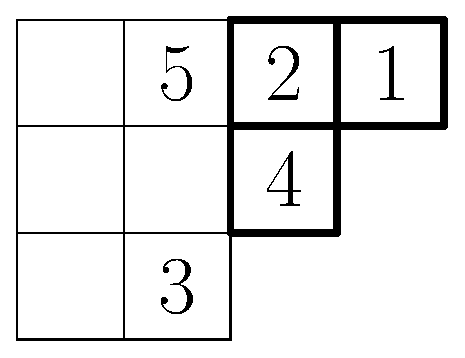
\includegraphics[scale=0.5]{Filling.eps}
%    \young(\hfil521,\hfil\hfil4,\hfil3)
    \caption{An example of a filling in the set $\mathcal{T}_{5,(2,1),3}$, which indexes the cells in the affine paving of $Y_{5,(2,1),3}$. The cell corresponding to this filling is not of maximal dimension because the entries outside $\lambda$ are not all in the bottom row and the $\lambda$ entries are not column-strict.}
    \label{fig:Filling}
\end{figure}

\begin{example}
Taking our basis of $\mathbb{C}^k$,
the cell in Figure~\ref{fig:Filling} is (under one convention for cell indexing) two-dimensional and given by the flags of the form
\begin{align*}
\langle f_{11} \rangle \subseteq
\langle f_{11}, f_{12}\rangle &\subseteq
\langle f_{11}, f_{12}, f_{31}+\alpha_1f_{21}+\alpha_2f_{13}\rangle \\
&\subseteq \langle f_{11}, f_{12}, f_{31}+\alpha_2f_{13}, f_{21} \rangle \\
& \subseteq \langle f_{11}, f_{21}, f_{31}, f_{21}, f_{13}\rangle,
\end{align*}
where $\alpha_1$ and $\alpha_2$ are arbitrary complex parameters.
\end{example}




\begin{lemma}
The cells in the affine paving, defined inductively from Lemma~\ref{lem:ProductIso}, are in bijection with $\mathcal{T}_{n,\lambda,s}$.
\end{lemma}




With appropriate choices of the isomorphisms in Lemma~\ref{lem:ProductIso} and indexing of the cells of $Y_{n,\la,s}$, it is possible to realize the affine paving as a restriction of the Schubert decomposition of $\Fl_{1,\dots,n}(\bC^m)$.

\begin{lemma}
Under an appropriate total ordering of the basis $\{f_{i,j}\}$ of $\bC^m$, the Schubert decomposition of $\Fl_{1,\dots n}(\bC^m)$ restricts to an affine paving of $Y_{n,\la,s}$ upon intersecting the Schubert cells with $Y_{n,\la,s}$. Precisely, the nonempty intersections of the form $C_w\cap Y_{n,\la,s}$, where $C_w$ is a Schubert cell, are the cells in an affine paving of $Y_{n,\la,s}$ that respects the isomorphisms in Lemma~\ref{lem:ProductIso}.
\end{lemma}

\begin{proof}[Proof of Theorem~\ref{thm:MainTheorem} (Sketch)]
First, we use the affine paving combined with Lemma~\ref{lem:OddCohVanishes} to show that the dimensions of the graded pieces of $H^*(Y_{n,\lambda,s};\bQ)$ and $R_{n,\lambda,s}$ are the same. Second, we show that the main theorem holds in the case $\lambda=\emptyset$,
\begin{align}
H^*(Y_{n,\emptyset,s};\bQ) \cong R_{n,\emptyset,s} = \frac{\bQ[x_1,\dots,x_n]}{\langle x_1^s,\dots, x_n^s\rangle}.
\end{align}
Third, we exhibit a surjective map on cohomology
\begin{align}\label{eq:CohSurj}
    \frac{\bQ[x_1,\dots, x_n]}{\langle x_1^s,\dots,x_n^s\rangle} \cong H^*(Y_{n,\emptyset,s};\bQ) \twoheadrightarrow H^*(Y_{n,\la,s};\bQ).
\end{align}
Finally, by combining a dimension counting argument and results of Brundan and Ostrik~\cite{Brundan-Ostrik} on Spaltenstein varieties, we show that the kernel of the surjection in \eqref{eq:CohSurj} is generated by the polynomials $e_d(S)\in I_{n,\lambda,s}$.
\end{proof}


\section{A Springer correspondence for induced Specht modules}\label{sec:InducedSpecht}


In this section, we characterize the irreducible components of $Y_{n,\la,s}$. In the case $s>\ell(\la)$, the number of irreducible components is equal to $\binom{n}{k}\cdot\#\SYT(\la)$.

Given a subspace $W\subseteq \bC^m$ such that $NW\subseteq W$, then $N(W\cap\bC^\lambda)\subseteq W\cap \bC^\lambda$. The nilpotent operator $N$ thus induces a nilpotent operator on the quotient space $\bC^\lambda/(W\cap \bC^\lambda)$, which we denote by $N|_{\bC^\lambda/(W\cap \bC^\lambda)}$.

Suppose $T$ is a filling of the Young diagram of $\lambda$ with a $k$-element subset of $[n]$ that decreases from left to right across each row. Let $T|_{n,\dots, n-i+1}$ be the restriction of $T$ to the cells containing the labels $n,\dots, n-i+1$. Furthermore, let $\mathrm{sh}(T|_{n,\dots, n-i+1})$ be the partition obtained by recording the row sizes of $T|_{n,\dots, n-i+1}$ and then sorting them to a partition.
Given such a filling $T$ that also decreases down each column, define the following subset of $Y_{n,\la,s}$,
\begin{align}
Y_{n,\la,s}^{T} = \{V_\bullet \in Y_{n,\la,s} \st N|_{\bC^\lambda/(V_i\cap \bC^\lambda)}\text{ has Jordan type }\mathrm{sh}(T|_{n,\dots,n-i+1})\text{ for all }i\}.
\end{align}


\begin{lemma}
\label{lem:Jordan}
Each subvariety $Y_{n,\la,s}^{T}$ is an irreducible locally-closed union of cells from the affine paving.
If $s>\ell(\la)$, then each $Y_{n,\la,s}^{T}$ is nonempty. If $s = \ell(\la)$, then $Y_{n,\la,s}^{T}$ is nonempty if and only if for all $i$, if $T$ does not contain $i$ as a label then the labels up to $i-1$ fill at least one row of $\lambda$. Furthermore, if $Y_{n,\la,s}^{T}$ is nonempty, then
\begin{align}\label{eq:DimFormulaForCmpt}
\dim_\bC(Y_{n,\la,s}^{T}) = n(\la) + (n-k)(s-1).
\end{align}
The $Y_{n,\la,s}^{T}$ give a partition of $Y_{n,\la,s}$ as we consider all possible choices for $T$.
\end{lemma}

\begin{theorem}
The space $Y_{n,\la,s}$ is equidimensional of dimension $n(\la) + (n-k)(s-1)$.  In particular, the closed subvarieties $\overline{Y_{n,\la,s}^{T}}$ for which $Y_{n,\la,s}^{T}$ is nonempty (as described in Lemma \ref{lem:Jordan}) form a complete set of irreducible components. In the case $s>\ell(\la)$, there are $\binom{n}{k}\cdot \#\SYT(\la)$ many irreducible components.
\end{theorem}

For each cell in the affine paving, the filling $T$ can be obtained from the partial filling of $\Lambda$ by restricting the labeling to the upper right copy of $\lambda$ contained in $\Lambda$, as depicted in Figure~\ref{fig:Lambda}.

\begin{example}
For the filling in Figure \ref{fig:Filling}, the corresponding filling of $\lambda$ is
\[\young(21,4),\]
and the Jordan types of the operators $N|_{\bC^\lambda/(V_i\cap \bC^\lambda)}$ for $i=1,2,3,4,5$ are
\[
{\small \yng(1,1)}\supset {\small \yng(1)}\supset {\small \yng(1)}\supset \emptyset \supset \emptyset.
\]
Notice that the filling was not column-strict; accordingly, the row lengths corresponding to the Jordan type of $N|_{\bC^\lambda/(V_2\cap \bC^\lambda)}$ are $(0, 1)$ (corresponding to the entry $4 \in \lambda$), but become $(1, 0)$ after sorting.
\end{example}

In the case $s>\ell(\la)$, the irreducible components are naturally indexed by Standard Young Tableaux on $(n-k) \cup \la$.  This indexing of irreducible components extends to a representation theory statement on the top cohomology group of $Y_{n,\lambda,s}$, generalizing Springer's theorem that the top cohomology group of a Springer fiber is a Specht module.
 

\begin{theorem}
Let $d = \dim(Y_{n,\la,s}) = n(\la) + (n-k)(s-1)$, and consider $S_k$ as the subgroup of $S_n$ permuting the elements of $[k]$. For $s>\ell(\la)$, we have an isomorphism of $S_n$-modules
\begin{align}
H^{2d}(Y_{n,\la,s};\bQ) \cong \mathrm{Ind}\!\uparrow_{S_k}^{S_n} (S^\la).
\end{align}
For $s=\ell(\la)$, we have
\begin{align}\label{eq:SLengthLambdaIso}
    H^{2d}(Y_{n,\la,s};\bQ) \cong S^{\Lambda/(n-k)^{s-1}},
\end{align}
the Specht module of skew shape $\Lambda/(n-k)^{s-1}$.
\end{theorem}

In the case of $s>\ell(\la)$, the proof follows by combining Theorem~\ref{thm:MainTheorem} and the fact that, in this case, the top degree component of $R_{n,\lambda,s}$ is isomorphic to $\mathrm{Ind}\!\!\uparrow_{S_k}^{S_n}(S^\lambda)$~\cite[Corollary 3.3.15]{GriffinThesis}. In the case of $s=\ell(\la)$, the proof follows by combining Theorem~\ref{thm:MainTheorem} with the formula \cite[Theorem 5.13]{GriffinOSP} for $\Frob(R_{n,\lambda,s};q)$ and then using bijective techniques to show that the top degree component of this symmetric function is the skew Schur function $s_{\Lambda/(n-k)^{s-1}}(x)$.






\section{Future work}\label{sec:FutureWork}

The $S_n$-module structure of the cohomology of a Springer fiber, $H^*(\cB^\lambda;\bQ)$, has several constructions. One construction involves utilizing the Grothendieck--Springer resolution and intersection cohomology, and it is known that this action is the same as the one defined by permuting the cohomology classes $-c_1(\widetilde V_i/\widetilde V_{i-1})$.

\begin{problem}
Find a generalization of the Grothendieck--Springer resolution, and realize the $S_n$-module structure on $H^*(Y_{n,\lambda,s};\bQ)$ defined in this article as a specialization of an $S_n$-action on an intersection cohomology complex.
\end{problem}


\begin{problem}
Find a generalization of the family of varieties $Y_{n,\lambda,s}$ to other Lie types such that the top cohomology groups gives an induced module analogue of the Springer correspondence in those types.
\end{problem}






\acknowledgements{
We are grateful to Sara Billey, Erik Insko, Isabella Novik, Julia Pevtsova, Martha Precup, Brendon Rhoades, and Andy Wilson for helpful conversations.
}

%% if you use biblatex then this generates the bibliography
%% if you use some other method then remove this and do it your own way
\printbibliography



\end{document}
